\chapter{페르미온의 부호와 초대칭 상쇄}

\lectureoverview{초대칭은 보손과 페르미온을 서로 연결하지만, 그런 관계를 원하는 이유는 그 대수적 구조를 쓰기 전에 살펴보면 더 쉽게 드러난다. 먼저 회전의 위상적 성질을 살펴보고, 간섭을 통해 페르미온 파동함수의 부호를 관측 가능하게 만든 다음, 교환 반대칭성에서 닫힌 페르미온 고리의 마이너스 부호를 유도한다. 이어서 보손 고리와 페르미온 고리의 부호가 서로 반대라는 점을 이용해 진공 에너지와 스칼라 자기 에너지의 상쇄를 설명한다. 후반부에서는 초대칭이 얼마나 깨져 있을 수 있는지, 초대칭 짝입자를 어떻게 검출할 수 있는지, 그리고 정확한 초대칭이 보통 원자의 전자껍질 구조를 왜 없애는지 묻는다.}

\section{초대칭에 앞서: 회전의 특이한 성질}

초대칭은 페르미온과 보손 사이의 대칭이다. 그러나 이를 구성하기에 앞서, 이 두 종류의 입자가 회전에 얼마나 다르게 반응하는지 되짚어 볼 만하다. 이 질문은 직접 보여 주기는 쉽지만, 한번 보고 나면 좀처럼 잊기 어려운 위상적 사실에서 시작한다.

한 손을 손바닥이 위를 향하게 들고 손목을 \(2\pi\)만큼 회전시켜 보자. 손은 처음 방향으로 돌아오지만, 팔은 분명 처음과 동등한 상태로 돌아오지 않았다. 팔이 꼬여 있기 때문이다. 팔을 움직여 가며 \(2\pi\)만큼 더 회전시키면 꼬임을 풀 수 있다. 따라서 주변을 고정한 채로는 \(2\pi\) 회전을 회전하지 않은 상태로 연속적으로 변형할 수 없지만, \(4\pi\) 회전은 그렇게 변형할 수 있다. 손으로 보여 주는 이 시연은 말 그대로 손을 움직여 보이는 증명이다.

해부학에 의존하지 않고도 같은 점을 보일 수 있다. 공을 고정된 상자 안에 넣고, 공을 상자 벽에 유연하고 늘어나지만 끊어지지 않는 줄을 몇 개든 이용해 연결하자. 공을 \(2\pi\)만큼 한 바퀴 회전시키면 줄이 얽히고, 줄만 움직여서는 원래 상태로 되돌릴 수 없다. 공을 총 \(4\pi\)만큼 회전시키면 줄을 공 주위로 움직여 얽힌 상태를 풀 수 있다. 상자 벽은 공간 무한대를 나타낸다. 공과 함께 경계도 회전시키지 않아야 비교가 의미를 갖는다.

\begin{classroomqa}\audiencequestion{상자를 회전시키면 얽힌 상태를 풀 수 있나요? \lecturetimestamp{00:02:53}}\lecturerresponse{그렇게 하면 문제가 달라집니다. 상자는 공간 무한대를 나타내므로 고정되어 있습니다. 여기서 비교하는 것은 물체와 주변 환경을 함께 회전시키는 것이 아니라, 주변 환경에 대해 물체를 회전시키는 경우입니다.}\end{classroomqa}

\begin{classroomqa}\audiencequestion{공을 \(2\pi\)만큼 더 회전시키면 안 되나요? \lecturetimestamp{00:03:20}}\lecturerresponse{바로 그 점이 두 경우를 구별합니다. 공을 더 회전시키지 않으면 \(2\pi\) 회전 뒤에 남은 얽힘을 풀 수 없습니다. 두 번째 회전을 마쳐 총 \(4\pi\) 회전하면 얽힘을 풀 수 있습니다.}\end{classroomqa}

현대적인 군론의 언어로 말하면, 회전군에는 닫힌 경로의 위상적 분류가 두 가지 있다:
\begin{equation}
\pi_1\!\left(SO(3)\right)\cong \mathbb Z_2.
\end{equation}
한 번 돌면 자명하지 않은 분류에 속하지만, 두 번 돌면 자명한 분류에 속한다.
다르게 말해 \(SU(2)\)는 \(SO(3)\)의 이중 피복이다. 이것이 페르미온 부호의 기하학적
선사(先史)다.

\editorialnote{\(SO(3)\), \(SU(2)\), 기본군이라는 언어를 사용하면 위상적 구조가 명시적으로 드러난다. 팔과 줄을 이용한 시연은 기하학적으로 같은 두 값의 거동을 보여 준다.}

\section{\texorpdfstring{\(2\pi\)}{ 회전이 양자 상태에 하는 일2}}

이제 입자의 위치를 고정하고, \(\ket{\psi}\)로 나타내는 스핀 상태만 남겨 두자. 정수 스핀 입자는 보손이고 반정수 스핀 입자는 페르미온이다. 강한 자기장 속에서 전하를 띤 스핀을 두고 자기장을 회전시키거나, 고정된 자기장 안에서 스핀이 원하는 각도만큼 세차운동하게 하면 물리적 회전을 구현할 수 있다.

\begin{classroomqa}\audiencequestion{실험실에서 전자 스핀을 실제로 어떻게 회전시키나요? \lecturetimestamp{00:05:26}}\lecturerresponse{자기장을 이용하면 됩니다. 스핀이 자기장을 따라가도록 충분히 강한 자기장을 회전시키거나, 고정된 자기장 주위로 스핀이 세차운동하게 할 수 있습니다. 전자를 손으로 잡아 돌리는 방법은 실험적으로 경쟁력이 없습니다.}\end{classroomqa}

\(2\pi\)만큼 한 바퀴 회전시키면 상태에 위상因자 하나가 곱해진다고 하자:
\begin{equation}
R(2\pi)\ket{\psi}=\xi\ket{\psi}.
\end{equation}
이 연산을 두 번 수행하면
\begin{equation}
R(4\pi)\ket{\psi}=\xi^2\ket{\psi}.
\end{equation}
\(4\pi\) 경로는 위상적으로 자명하므로, 이 비교에서 항등 연산으로 작용해야 한다. 따라서
\begin{equation}
\xi^2=1,
\qquad
\xi=+1\ \hbox{or}\ -1.
\end{equation}
보손은 플러스 부호를, 페르미온은 마이너스 부호를 갖는다:
\begin{align}
R(2\pi)\ket{\psi_B}&=+\ket{\psi_B},\\
R(2\pi)\ket{\psi_F}&=-\ket{\psi_F}.
\end{align}
스핀 \(j\)가 확정된 상태라면 간결하게 다음과 같이 쓸 수 있다.
\begin{equation}
R(2\pi)=(-1)^{2j}.
\end{equation}
강의 녹취에서는 두 번째 가능성이 \(2\pi\)를 곱하는 경우라고 잠시 말하지만, 이어지는 유도와 판서의 논증을 보면 의도한 인자는 \(-1\)임을 알 수 있다.

처음에는 이것이 물리적으로 아무 의미도 없어 보인다. 파동함수 전체의 부호가 바뀌더라도
\begin{equation}
\Psi\longmapsto-\Psi,
\end{equation}
확률은 바뀌지 않는다. 왜냐하면
\begin{equation}
(-\Psi)^*(-\Psi)=\Psi^*\Psi.
\end{equation}
동일한 상태로 준비한 전자 앙상블 두 개를 생각하자. 한 앙상블의 모든 전자를 \(2\pi\)만큼 회전시키고 다른 앙상블은 그대로 둔다. 고립된 전자 하나에 대한 어떤 측정으로도 그 전자가 어느 앙상블에서 왔는지 알아낼 수 없다. 전체 위상은 관측 가능한 양이 아니다.

\section{마이너스 부호를 상대 위상으로 만들기}

파동함수의 간섭성 있는 한 갈래에만 부호 변화를 주고 다른 갈래에는 주지 않으면 그 부호를 관측할 수 있다. 두 경로 장치를 통해 전자를 한 번에 하나씩 보내자. 어느 경로를 지나는지 알아내지는 말자. 경로 정보를 얻으면 간섭이 사라지기 때문이다. 위쪽과 아래쪽 경로의 진폭을 각각 \(\psi_1\)와 \(\psi_2\)라 하면, 두 경로가 다시 합쳐진 상태는 다음과 같다.
\begin{equation}
\Psi=\psi_1+\psi_2.
\end{equation}
잠시 각 경로를 자기장 영역에 가두었다고 하자. 두 번째 경로에 해당하는 자기장만 \(2\pi\)만큼 회전시킨다. 입자가 페르미온이면 상태는 다음과 같이 된다.
\begin{equation}
\Psi'=\psi_1-\psi_2.
\end{equation}
이제 부호 변화는 전체에 공통으로 적용되지 않는다. 상대 위상이 바뀌어 간섭 무늬의 극대와 극소가 서로 뒤바뀐다. 검출기 중앙을 기준으로 두 입사 파동묶음이 서로 거울상이라면 반대칭 조합은 중앙에서 상쇄된다:
\begin{equation}
\Psi'(0)=\psi_1(0)-\psi_2(0)=0.
\end{equation}
따라서 전자는 이 대칭점에서 검출되지 않는다. 두 경로를 모두 회전시키면 대신 \(-\psi_1-\psi_2=-\Psi\)가 되며, 이는 관측 가능한 효과를 내지 않는다.

강의에서는 이 실험의 상대적 성격을 강조한다. 한 자기장 영역을 다른 영역에 대해 회전시키는 것은 상자는 고정한 채 공을 회전시키는 것과 비슷하다. 두 영역을 함께 회전시키는 것은 공과 상자를 함께 회전시키는 것과 비슷하다. 상대적으로 \(4\pi\)만큼 회전하면 페르미온 상태가 플러스 부호를 띠며 되돌아오기 때문에 효과가 사라진다. 강의에서 잠깐 언급하듯 이 실험은 Yakir Aharonov와 Leonard Susskind가 1967년에 제안했으며, 나중에 간섭계 방식으로 구현되었다. 같은 원리를 전자나 전하를 띤 이온에 적용할 수 있다. 간섭 무늬의 이동은 반정수 스핀 상태를, 무늬가 이동하지 않는 것은 정수 스핀 상태를 나타낸다.

\begin{classroomqa}\audiencequestion{상대 자기장을 \(4\pi\)만큼 회전시키면 이동한 무늬가 원래 상태로 돌아오나요? \lecturetimestamp{00:12:21}}\lecturerresponse{그렇습니다. 부호 변화 두 번을 곱하면 \(+1\)가 되므로, 극대와 극소를 서로 바꾸던 상대 위상이 사라집니다.}\end{classroomqa}

\begin{classroomqa}\audiencequestion{상자 속 줄을 페르미온과 얼마나 문자 그대로 연결해 생각해야 하나요? \lecturetimestamp{00:13:43}}\lecturerresponse{그 줄은 위상을 이해하기 위한 비유이지, 전자에 실제로 매달린 물리적 줄이 아닙니다. 보손은 \(2\pi\) 회전 뒤에 흔적이 남지 않는 것처럼 거동하고, 페르미온은 자명하지 않은 얽힘이 나타내는 부호의 흔적을 그대로 유지합니다.}\end{classroomqa}

\begin{classroomqa}\audiencequestion{두 자기장 영역에 전자가 하나씩, 모두 두 개 있어서 하나는 회전하고 다른 하나는 그대로인가요? \lecturetimestamp{00:14:29}}\lecturerresponse{아닙니다. 간섭성 있는 공간 중첩 상태에 전자 하나가 있습니다. 전자는 각 경로에 있을 진폭을 가지며, 장치가 전자가 어느 경로에 있었는지 드러내서는 안 됩니다. 한 영역만 회전시키면 한 진폭이 다른 진폭에 대해 달라지고, 두 영역을 모두 회전시키면 공통 위상만 바뀝니다.}\end{classroomqa}

각도 \(2\pi\)가 특별한 이유는 스핀 방향은 원래대로 돌아오지만 스피너에는 부호가 생기기 때문이다. 일반적인 상대 회전에서는 스핀 방향도 바뀐다. 두 경로 상태가 각각 스핀 상태 \(\ket{\chi_1}\)와 \(\ket{\chi_2}\)로 돌아온다면 간섭항은 다음에 비례한다.
\begin{equation}
\braket{\chi_1}{\chi_2}.
\end{equation}
그 크기가 간섭 무늬의 가시도를 결정한다.\editorialnote{스핀 내적 식은 부분적 또는 완전한 간섭 소실에 관한 강의의 정성적 설명을 표준적인 형태로 보완한 것이다.}서로 직교하는 스핀 상태는 경로 정보를 완전히 담고 있으므로 간섭하지 않는다.

\begin{classroomqa}\audiencequestion{어느 자기장 영역에 전자가 있었는지 측정하면 어떻게 되나요? \lecturetimestamp{00:18:03}}\lecturerresponse{간섭 무늬가 사라집니다. 두 경로를 구별하는 어떤 기록이든 진폭의 간섭성 있는 합을 없앱니다.}\end{classroomqa}

\begin{classroomqa}\audiencequestion{모든 스핀이 같은 방향에서 시작하고 마지막 스핀을 측정한다면, \(2\pi\) 연산 자체가 그 방향을 바꾸나요? \lecturetimestamp{00:18:17}}\lecturerresponse{아닙니다. \(2\pi\) 회전 뒤에도 물리적인 스핀 방향은 같습니다. 바뀐 것은 페르미온 경로에 마이너스 부호가 붙었다는 점뿐입니다. 따라서 이 연산은 경로를 표시할 정도로 스핀 방향을 바꾸지 않고도 간섭을 바꿀 수 있습니다.}\end{classroomqa}

\begin{classroomqa}\audiencequestion{자기장을 \(\pi\)만큼만 회전시키고 \(2\pi\)만큼은 회전시키지 않으면 어떻게 되나요? \lecturetimestamp{00:18:43}}\lecturerresponse{그러면 스핀 방향이 바뀝니다. 위쪽 스핀 경로와 아래쪽 스핀 경로는 서로 구별되므로 간섭할 수 없습니다. 중간 각도에서는 가시도가 연속적으로 낮아지고, 상대적으로 \(180^\circ\)만큼 회전하면 간섭이 완전히 사라집니다.}\end{classroomqa}

\section{교환 대칭성과 닫힌 고리의 부호}

회전에 관한 논의에서는 페르미온의 마이너스 부호 하나를 확인했다. 동일 입자를 교환할 때도 이와 밀접하게 관련된 또 다른 부호가 나타난다. 두 입자 파동함수에 대해
\begin{align}
P_{12}\Psi_B(1,2)&=+\Psi_B(1,2)=+\Psi_B(2,1),\\
P_{12}\Psi_F(1,2)&=-\Psi_F(1,2)=-\Psi_F(2,1).
\end{align}
보손 상태는 대칭이고 페르미온 상태는 반대칭이다.

\begin{figure}[htbp]\centering
\includegraphics[width=0.74\textwidth]{lecture_02_figure_02.png}\lectureframe{00:24:27}\caption{상태 표기로 나타낸 교환 논증. 영상에서 판독 가능한 것은 켓 표기뿐이며, 반대칭성 방정식은 흐릿한 판서에 있다고 주장하지 않고 본문에 조판했다.}\end{figure}

이제 적분을 계산하지 않고도 닫힌 입자 고리의 상대 부호를 알아낼 수 있다. 외부 다리가 없는 진공 페인먼 도표를 생각하자. 이를 시공간에서 입자가 닫힌 경로를 따라가는 모습으로 그리거나, 입자와 반입자 쌍이 생성되었다가 나중에 소멸하는 모습으로 그릴 수 있다. 이런 진공 도표는 진공 진폭, 따라서 진공 에너지에 기여한다.

서로 연결되지 않은 고리 두 개에서 시작하자. 연결되지 않은 도표의 기여는 서로 곱해지므로, 고리 하나의 부호가 \(\sigma\)이면 두 고리의 부호는
\begin{equation}
\sigma^2=+1.
\end{equation}
두 고리를 같은 시각, 예를 들어 \(t=0\)에서 자르자. 그 순간에는 동일 입자 두 개가 있다. 입자를 교환하지 않고 다시 연결하면 두 개의 분리된 고리가 되돌아온다. 다시 연결하기 전에 두 입자를 교환하면 위상 구조가 고리 하나로 바뀐다. 이 교환은 보손의 경우 \(+1\), 페르미온의 경우 \(-1\)을 곱한다. 처음 두 고리의 부호가 양수였으므로, 결과로 얻는 한 고리의 부호는 다음과 같다.
\begin{equation}
\begin{aligned}
\operatorname{sign}(\text{closed boson loop})&=+1,\\
\operatorname{sign}(\text{closed fermion loop})&=-1.
\end{aligned}
\end{equation}
더 일반적으로 서로 독립적인 닫힌 페르미온 고리가 \(L_F\)개인 도표에는 다음 인자가 붙는다.
\begin{equation}
(-1)^{L_F}.
\end{equation}
강의에서는 그라스만 적분을 바로 언급하는 대신 교환을 이용해 이 규칙을 의도적으로 유도한다. 이 간단한 논증은 부호의 물리적 기원을 드러낸다.

\section{반대 부호의 고리와 진공 에너지}

보손 진공 고리는 한 부호로 진공 기여를 증가시키고, 페르미온 고리는 반대 부호로 기여한다. 이는 곧바로 양자장론의 순진한 절단 추정값에 비해 관측된 암흑 에너지 밀도가 극히 작다는 사실을 떠올리게 한다. 강의에서는 악명 높은 불일치가 대략 \(123\)자릿수라고 말한다. 정확한 지수는 어떤 자외선 척도를 택하느냐에 따라 달라지지만, 엄청난 불일치가 있다는 점은 변하지 않는다.

고리 보정의 값은 통계적 성질만으로 결정되지 않는다. 질량, 전하, 중복도, 상호작용에도 좌우된다. 그러나 보손과 페르미온이 관련된 모든 성질에서 서로 대응하면, 크기가 같은 두 기여가 상쇄될 수 있다:
\begin{equation}
\begin{gathered}
m_B=m_F,\qquad q_B=q_F,\qquad g_B=g_F,\\
\Delta\rho_{\mathrm{vac}}^{(B)}
+\Delta\rho_{\mathrm{vac}}^{(F)}=0.
\end{gathered}
\end{equation}
이 관찰만으로 우주상수 문제를 해결할 수 있는 것은 아니다. 다만 보손 고리 보정만으로는 얻을 수 없었던 반대 부호의 기여를 제공한다. 적절한 가정 아래 정확히 깨지지 않은 전역 초대칭 이론에서는 진공 에너지의 상쇄가 실제로 정확할 수 있다. 초대칭이 깨진 뒤에도 관측된 극히 작으면서도 영은 아닌 값은 여전히 설명되지 않는다.\editorialnote{이 단서는 강의의 동기와 훨씬 더 어려운 우주상수 문제를 구분해 준다.}

이미 정확한 대응이 자연을 설명하지 못한다는 점은 알려져 있다. 전자와 질량 및 전하가 같은 스핀 0 짝입자가 있다면, 가상 광자를 거치는 전자·양전자 소멸로 이 입자 쌍을 만들 수 있다:
\begin{equation}
e^-e^+\longrightarrow\gamma^*
\longrightarrow\widetilde e^-\widetilde e^+.
\end{equation}
질량이 같은 전하를 띤 스칼라 입자라면 일반적인 충돌기 실험에서 발견되지 않은 채 남아 있지 못했을 것이다. 따라서 보손과 페르미온 사이의 대응은 관측된 입자 스펙트럼의 정확한 대칭일 수 없다. 이는 입자 종류 사이의 대응이지, 물리적 공간에서의 반사가 아니다.

\section{더 직접적인 표적: 스칼라 자기 에너지}

진공 에너지는 첫 번째 사례일 뿐이며, 강의의 주된 관심은 스칼라 질량의 복사 불안정성이다. 처음에 맨질량이 0인 스칼라도 이차적으로 절단 척도에 의존하는 보정을 받을 수 있다. 개략적으로 보손 고리는 다음과 같은 기여를 한다.
\begin{equation}
\Delta m_H^2\sim \frac{g_B^2}{16\pi^2}\Lambda^2
\end{equation}
페르미온 질량은 다른 방식으로 보호된다. 질량이 없는 페르미온에 정확한 카이랄 대칭이 있으면, 복사 보정으로 가산적인 질량항이 생길 수 없다. 이것이 앞 강의에서 다룬 좌우 대칭 논증이다.

이제 스칼라와 페르미온을 하나의 다중항에 넣고 상호작용도 대응시킬 만큼 강한 대칭을 생각해 보자. 페르미온 고리는 반대 부호로 나타난다:
\begin{equation}
\Delta m_H^2
\sim
\frac{g_B^2-g_F^2}{16\pi^2}\Lambda^2+\cdots .
\end{equation}
초대칭이 \(g_B=g_F\)와 질량의 일치를 강제하면 이차항이 상쇄된다. 그리하여 페르미온을 보호하는 메커니즘이 그 보손 짝입자에게도 전달된다. 이는 두 도표의 수치가 우연히 맞아떨어지는 일이 아니다. 모든 차수와 허용된 모든 상호작용에서 대칭이 상쇄를 강제해야 한다.

칠판 전체를 가로지르는 비교 그림은 강의가 개별 고리에서 전파하는 입자의 짝지어진 고리 보정으로 넘어가는 모습을 보여 준다.

\begin{figure}[htbp]
\centering
\includegraphics[width=0.79\textwidth]{lecture_02_figure_04.png}
\lectureframe{00:40:23}

\medskip
\begin{tikzpicture}[scale=0.9]
\draw (-4.2,0) circle (0.55);
\draw[dashed] (-2.4,0) circle (0.55);
\draw (0,0) -- (3.7,0);
\fill (1.85,0) circle (0.055);
\draw (1.85,0) -- (1.85,0.25);
\draw[dashed] (1.85,0.85) circle (0.6);
\end{tikzpicture}\caption{보통 입자와 초대칭 짝입자의 고리 위상 구조를 칠판 전체에 걸쳐 비교한 그림. 조판된 그림은 눈에 보이는 위상적 차이만 보존하며, 흐릿한 입자 표기는 특정하지 않는다.}\end{figure}

강의실 휴식 후 논의는 이른바 영차 근사 그림에서 다시 시작한다. 여기서 영차는 섭동 이론의 차수를 뜻하지 않는다. 유용한 설명 가운데 가장 개략적인 것을 뜻한다:
\begin{quote}
모든 입자에는 통계적 성질이 반대인 초짝입자가 있다. 모든 페르미온에는 보손 짝입자가 있고, 모든 보손에는 페르미온 짝입자가 있다.
\end{quote}
정확한 초대칭 이론에서는 짝입자들의 질량도 같아 축퇴되어 있을 것이다. 자연은 이런 식으로 축퇴되어 있지 않다. 그래도 질량이 서로 다르더라도 그 차이가 지나치게 크지 않다면, 폭발적으로 큰 스칼라 질량 보정을 막을 만큼 상쇄가 충분히 잘 유지될 수 있다. 연성 초대칭 깨짐이 있으면 위험한 에너지 척도는 개략적으로 초짝입자 질량의 분열로 대체된다:
\begin{equation}
\Delta m_H^2\sim
\frac{g^2}{16\pi^2}\,\Delta m_{\mathrm{SUSY}}^2
\ln\!\frac{\Lambda^2}{\Delta m_{\mathrm{SUSY}}^2}
\end{equation}
모형에 따라 달라지는 계수는 생략했다.\editorialnote{이 식은 질량이 완벽히 대응하지 않을 때 남는 보정이 질량 분열에 의해 좌우된다는 강의의 정성적 설명을 나타내며, 칠판의 식을 옮긴 것은 아니다.}

\section{초대칭 깨짐과 2010년의 실험적 기대}

이 강의가 녹화된 2010년 당시에는 초대칭 짝입자가 하나도 관측되지 않았다. 따라서 짝입자가 실제로 존재한다면 알려진 입자보다 무거워야 하고, 이전 가속기의 도달 범위를 넘어서는 질량을 가져야 한다고 바로 추론했다. 초대칭 모형은 또 질량이 전약 대칭 깨짐 뒤에야 생기는 입자와 대칭을 보존하면서 더 큰 질량을 가질 수 있는 상태를 구별한다. 강의에서는 이를 근거로 초대칭 스펙트럼에서 관측 가능한 쪽은 가벼울 수 있고 보이지 않는 쪽은 더 무거울 수 있다고 설명하면서도, 이런 구성이 무리한 가정임을 솔직히 인정한다. Susskind는 초대칭 짝입자가 검출될 것이라는 자신의 기대를 밝힌 직후, 그것은 결과가 아니라 추측이라고 분명히 한다.

따라서 대형 강입자 충돌기는 강의가 전망한 실험에서 핵심적인 역할을 했다. 이 충돌기는 힉스 보손과 초대칭 짝입자를 모두 찾을 것으로 기대되었다. 이 발언은 2010년이라는 시대적 맥락에서 읽어야 한다. 강의는 힉스 발견과 그 이후의 LHC 탐색 결과가 나오기 전의 실험적 기대를 설명하고 있다.

자연성에 근거해 도입한 초대칭 짝입자가 플랑크 척도에 있어서는 왜 안 되는가? 그렇게 되면 그 짝입자에 맡긴 역할을 해내지 못하기 때문이다. 보손과 페르미온의 질량 차이가 엄청나면, 가벼운 쪽의 질량을 넘는 에너지에서 두 고리 적분은 더 이상 상쇄되지 않는다. 남는 스칼라 보정의 크기는 대략 약한 상호작용 척도가 아니라 무거운 쪽의 질량 분할로 정해진다. 임의로 먼 에너지 척도의 초대칭도 수학적 대칭일 수는 있지만, 가벼운 힉스 부문을 설명하는 설득력은 더 이상 없다.

강의에서는 이를 당시의 기대에 맞춰, 관련 질량 분할이 대략 수백 GeV 이내라서 LHC가 도달할 수 있어야 한다고 설명한다. 이 수치 추정은 당시의 것이며 모형에 따라 달라진다. 더 중요한 것은 다음 논리의 흐름이다:
\begin{equation}
\begin{gathered}
\text{Higgs protection}\\
\Downarrow\\
\text{effective boson--fermion cancellation}\\
\Downarrow\\
\Delta m_{\mathrm{SUSY}}\ \text{not too large}.
\end{gathered}
\end{equation}

\begin{classroomqa}\audiencequestion{페르미온 기여 전체와 보손 기여 전체가 서로 일대일 짝입자 없이도 합계로 상쇄될 수 있나요? \lecturetimestamp{00:45:01}}\lecturerresponse{수치상 상쇄될 수는 있지만, 그것은 원래 문제만큼이나 정밀하게 맞춰야 하는 우연한 상쇄일 것입니다. 초대칭 가설은 그보다 강합니다. 합리적인 가정만으로 대응하는 기여가 일치하도록 강제하고, 초대칭 깨짐은 질량이 근사적으로만 일치하는 이유를 설명합니다. 여기서 진공 에너지는 예시였고, 당장의 관심사는 힉스 자기 에너지입니다.}\end{classroomqa}

\begin{classroomqa}\audiencequestion{합계의 상쇄를 부자연스럽다고 부르는 것 자체가 이론을 환원주의적으로 구성한다고 이미 가정하는 것은 아닌가요? \lecturetimestamp{00:47:51}}\lecturerresponse{타당한 지적입니다. 자연성에 대한 최종적인 정의를 내린 사람은 없고, 이 탐색은 설득력 있는 설명을 더듬어 찾는 과정이기도 합니다. 초대칭과 자발적 초대칭 깨짐은 원하는 양상을 강제할 수 있는 알려진 수학적 틀을 제공합니다. 해결되지 않은 질문은 자연이 실제로 그 틀을 사용하는지, 그리고 그 틀이 유일한지입니다.}\end{classroomqa}

\section{직접 생성, 가상 효과, 붕괴 연쇄}

무거운 입자가 실험에 영향을 주려면 질량 껍질 위에서 생성되어야 하는 것은 아니다. 입자는 고리 안에 가상적으로 나타나 보통의 전자·양전자 산란 진폭을 조금 바꿀 수 있다. 따라서 중심 질량 에너지가 직접 쌍생성 문턱보다 낮아도 정밀 전약 측정으로 초대칭 짝입자의 존재를 제한할 수 있다.
\begin{equation}
\sqrt{s}<2m_{\widetilde p}.
\end{equation}
강의에서 2010년 당시 내린 평가는 정밀 측정 자료가 이미 초대칭 모형의 매개변수 공간을 좁히고 있었지만, 초대칭을 배제하지는 못했다는 것이다.

\begin{classroomqa}\audiencequestion{이전의 무거운 입자들을 직접 관측하기 전에 정밀한 생성률로 제약했듯이 초대칭 짝입자도 간접적으로 추론할 수 있나요? \lecturetimestamp{00:49:01}}\lecturerresponse{그렇습니다. 가상 초대칭 짝입자 고리가 보통의 진폭을 조금 바꾸므로, 문제는 직접 생성이 아니라 고정밀 전약 현상론이 됩니다. 충분한 에너지를 갖춘 깨끗한 전자·양전자 충돌기는 특히 유용할 것입니다. 양성자는 쿼크와 글루온으로 이루어진 복합 입자라 양성자 충돌은 더 복잡합니다. 초기 조건을 정확히 아는 두 기본 입자를 충돌시키는 것이 아니라, 요동하는 구성 성분들을 실제로 충돌시키기 때문입니다.}\end{classroomqa}

한 학생이 초입자를 풍부하게 가지고 있는 경우를 상정해 반대 방향으로 반응을 진행할 수 있는지 묻는다. 장애물은 시간 반전 대칭이 아니라 초입자의 확보 가능성이다. 무거운 초대칭 짝입자는 먼저 생성되어야 하고, 대부분은 더 가벼운 상태로 빠르게 붕괴할 것으로 예상된다.

\begin{classroomqa}\audiencequestion{우주에 초입자가 많이 있다면, 그중 둘이 충돌해 보통 입자로 바뀔 수 있나요? \lecturetimestamp{00:53:43}}\lecturerresponse{원리상 관련 반응에는 역반응 채널이 있지만, 무거운 초대칭 짝입자가 자유롭게 많이 남아 있을 것으로 예상되지는 않습니다. 이들은 더 낮은 에너지 상태로 붕괴하므로, 실험에서 먼저 충분한 충돌 에너지를 공급해 이들을 생성해야 합니다.}\end{classroomqa}

이로써 암흑물질 문제가 제기된다. 많은 초대칭 모형에서는 이산 선택 규칙 때문에 붕괴 연쇄의 마지막 초대칭 짝입자가 완전히 사라지지 않는다. 그러면 더 무거운 초대칭 짝입자는 모두 가장 가벼운 초대칭 짝입자, 즉 LSP를 향해 연쇄적으로 붕괴한다. LSP가 전기적으로 중성이라면 안정할 수 있고 검출하기 어려워 암흑물질 후보가 될 수 있다. 녹취록은 이 대화에서 한 번 암흑 에너지라고 말하지만, 청중의 질문과 입자에 대한 설명은 암흑물질을 명백히 가리킨다.

\begin{classroomqa}\audiencequestion{초대칭 짝입자가 빠르게 붕괴한다는 사실은 초대칭 짝입자가 암흑물질일 수 있다는 가설과 충돌하나요? \lecturetimestamp{00:54:53}}\lecturerresponse{아닙니다. 붕괴 연쇄의 끝에 초대칭 짝입자가 남도록 하는 모형에서는 대부분의 초대칭 짝입자가 붕괴하더라도 가장 가벼운 입자는 안정할 수 있습니다. 전하를 띠면 현상론적으로 추가 문제가 생기는 경우가 보통이므로, 가능한 LSP는 중성일 가능성이 높습니다. 원리상 검출할 수 없는 것은 아니지만, 전하를 띤 셀렉트론처럼 이온화 흔적을 뚜렷이 남기지는 않습니다.}\end{classroomqa}

\section{대응하려면 결합 상수도 일치해야 한다}

질량만 맞추는 것으로는 충분하지 않다. 전자 진공 고리와 셀렉트론 고리를 비교해 보자. 두 입자의 통계적 성질이 반대이므로 부호도 반대지만, 크기가 같으려면 질량이 같아야 한다. 이제 외부 광자 두 개를 붙여 보자. 계수에는 전자기 결합 상수도 들어가므로 상쇄하려면 전하도 같아야 한다:
\begin{equation}
\begin{gathered}
q_{\widetilde e}=q_e,\\
\mathcal A_{\mathrm{loop}}^{(e)}
+\mathcal A_{\mathrm{loop}}^{(\widetilde e)}=0,\\
\text{provided the full couplings match.}
\end{gathered}
\end{equation}
어느 단계에서든 대응이 어긋나면 발산하는 항이 상쇄되지 않고 남는다. 초대칭이 유용한 까닭은 입자의 이름이나 스핀뿐 아니라 상호작용도 서로 연결하기 때문이다.

\begin{figure}[H]
\centering
\includegraphics[width=0.66\textwidth]{lecture_02_figure_05.png}
\lectureframe{00:57:15}

\medskip
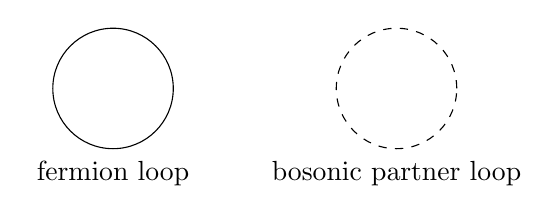
\begin{tikzpicture}[scale=0.9]
\draw (-2.0,0) circle (0.85);
\draw[dashed] (2.0,0) circle (0.85);
\node at (-2.0,-1.2) {fermion loop};
\node at (2.0,-1.2) {bosonic partner loop};
\end{tikzpicture}\caption{전하 대응 논증에서 비교한 실선과 점선 고리. 잘린 외부 표시는 그림만으로 모든 연결 지점을 알 수 없으므로 복원하지 않았다.}\end{figure}

\begin{classroomqa}\audiencequestion{초대칭 짝입자의 결합 상수가 다르기 때문에 검출을 피했을 수도 있나요? \lecturetimestamp{00:56:23}}\lecturerresponse{같은 도표들이 상쇄되어야 한다면 그럴 수 없습니다. 광자 상호작용을 더하면 각 선의 전하를 시험하게 됩니다. 결합 상수가 다르면 수치적인 고리 인자가 달라져 큰 잔여항이 다시 생깁니다. 대칭은 해당 전하와 상호작용을 서로 맞춰야 합니다.}\end{classroomqa}

\begin{classroomqa}
\audiencequestion{광자의 초짝입자도 질량이 없어야 하나요? \lecturetimestamp{00:58:01}}
\lecturerresponse{정확한 초대칭 이론에서는 광자와 질량이 같아 축퇴되어 있으므로 질량이 없을 것이다. 관측되는 세계는 정확한 초대칭을 따르지 않으므로, 실제 포티노와 유사한 상태의 질량이 광자의 질량과 같을 필요는 없다.}
\end{classroomqa}

\section{초대칭 짝입자 이름표}

이름 붙이는 규칙은 우아하지는 않지만 쓸모가 있다. 보손의 페르미온 짝입자 이름은 흔히 \emph{-ino}로 끝난다. 광자와 포티노, \(W\)와 위노, \(Z\)와 지노, 글루온과 글루이노, 힉스와 힉시노, 중력자와 중력자는 이런 쌍을 이룬다. 보통 페르미온의 보손 짝입자 이름은 대개 \emph{s-}로 시작한다. 전자와 셀렉트론, 쿼크와 스쿼크가 그 예다.

\begin{center}
\begin{tabular}{@{}>{\raggedright\arraybackslash}p{0.40\linewidth}>{\raggedright\arraybackslash}p{0.52\linewidth}@{}}
\toprule
일반 상태 & 초대칭짝과 스핀 변화\\
\midrule
스칼라 힉스, \(j=0\) & 힉시노, \(j=\tfrac12\); \(\Delta j=+\tfrac12\)\\
게이지 보손, \(j=1\) & 게이지노, \(j=\tfrac12\); \(\Delta j=-\tfrac12\)\\
물질 페르미온, \(j=\tfrac12\) & 스페르미온, \(j=0\); \(\Delta j=-\tfrac12\)\\
중력자, \(j=2\) & 중력자노, \(j=\tfrac32\); \(\Delta j=-\tfrac12\)\\
\bottomrule
\end{tabular}
\end{center}

일반적으로 초다중항의 구성원들은 스핀이 서로 반 단위만큼 다릅니다:
\begin{equation}
\Delta j=\frac12.
\end{equation}
강의에서 든 대략적인 예에서는 스핀 \(\tfrac12\)인 물질 페르미온과 스칼라 입자를 짝짓고, 스핀 1인 게이지 보손과 스핀 \(\tfrac12\)인 게이지노를 짝짓습니다. 완전한 상호작용 모형에서는 대칭성 깨짐 뒤에 상태들이 서로 섞일 수 있으므로, 물리적인 질량 고유상태가 이러한 가장 단순한 명칭을 그대로 따를 필요는 없습니다.

\begin{classroomqa}
\audiencequestion{새로운 스칼라 초대칭짝들이 모두 저마다 자발적인 대칭성 깨짐을 일으킬 수 있나요? \lecturetimestamp{01:01:27}}
\lecturerresponse{스칼라장은 기댓값을 가질 수 있지만, 임의의 추가 대칭성 깨짐은 현상론적으로 치명적일 것입니다. 실현 가능한 초대칭 모형은 스칼라 퍼텐셜을 적절히 구성하여 색, 전하 및 그 밖의 필요한 대칭성이 바람직하지 않은 방식으로 깨지지 않도록 해야 합니다.}
\end{classroomqa}

\begin{classroomqa}
\audiencequestion{힉스 사차항에 대응하는 특별한 상호작용이 힉시노에도 있는가? \lecturetimestamp{01:02:19}}
\lecturerresponse{초대칭에서는 입자뿐 아니라 상호작용도 서로 대응한다. 이 관계는 모든 힉스 선을 힉시노 선으로 기계적으로 바꾸는 식으로 얻어지는 것은 아니지만, 스칼라 사차항과 관련된 페르미온 및 보조장 상호작용은 하나의 제약된 구조에 속한다. 이 강의에서는 아직 그러한 세부 사항을 다루지 않았다.}
\end{classroomqa}

\begin{classroomqa}
\audiencequestion{\(2\pi\) 회전과 \(4\pi\) 회전에 관한 정리는 다른 차원에도 유사한 형태로 성립하나요? \lecturetimestamp{01:03:07}}
\lecturerresponse{그렇습니다. 다만 차원에 따라 가능한 경우가 달라집니다. 공간 차원이 2인 경우에는 교환 경로가 서로를 감아 돌 수 있어, 보손의 \(+1\) 및 페르미온의 \(-1\)보다 더 일반적인 교환 위상을 갖는 애니온이 가능합니다. 이런 들뜸은 응집물질계에서 나타나지만, 현재 강의의 흐름에서는 다루지 않습니다.}
\end{classroomqa}

\section{초대칭이 정확하면 화학은 사라진다}

이제 정확한 초대칭 세계가 어떤 모습일지 살펴보겠습니다. 여기서 정확하다는 말은 모든 입자와 초대칭짝의 질량이 같고 상호작용이 서로 대응한다는 뜻입니다. 전자는 질량과 전하가 같은 보손 셀렉트론을 가지며, 질량이 없는 광자는 질량이 없는 페르미온 포티노를 가집니다:
\begin{equation}
m_{\widetilde e}=m_e,
\qquad
q_{\widetilde e}=q_e,
\qquad
m_{\widetilde\gamma}=m_\gamma=0.
\end{equation}

화학의 익숙한 주기적 구조는 페르미 통계에 달려 있습니다. 수소 원자는 가장 낮은 궤도에 전자 하나를 가집니다. 헬륨 원자는 스핀 상태가 서로 달라 그 궤도에 전자 둘을 수용합니다. 리튬의 세 번째 전자는 더 높은 궤도에 놓여야 합니다. 파울리 배타 원리는 서로 구별할 수 없는 전자 세 개가 하나의 동일한 입자 상태를 차지하지 못하게 하기 때문입니다. 바깥쪽 전자는 에너지가 더 높으므로 안쪽으로 떨어지려 하며, 보통은 광자를 방출하겠지만, 아래쪽 상태가 이미 채워져 있어 그 전이가 막힙니다.

정확한 초대칭에서는 또 다른 경로가 열립니다:
\begin{equation}
e^-_{\mathrm{outer}}
\longrightarrow
\widetilde e^-_{\mathrm{inner}}
+
\widetilde\gamma .
\end{equation}
처음의 전자와 방출되는 포티노는 페르미온이고, 남은 셀렉트론은 보손입니다. 셀렉트론은 페르미 통계가 아니라 보스 통계를 따르므로, 마지막 셀렉트론은 이미 점유된 낮은 궤도에 들어가는 것이 금지되지 않습니다. 따라서 원자가 전자는 다른 입자로 바뀌어 안쪽으로 떨어질 수 있습니다.

\begin{figure}[H]
\centering
\includegraphics[width=0.62\textwidth]{lecture_02_figure_06.png}
\lectureframe{01:09:18}

\medskip
\begin{tikzpicture}[scale=0.9]
\fill (0,0) circle (0.075);
\draw (0,0) circle (0.72);
\draw (0,0) circle (1.45);
\draw[-{Latex[length=2.2mm]}] (1.42,0.2) .. controls (1.2,0.52) and (0.92,0.42) .. (0.72,0.1);
\draw[decorate,decoration={snake,amplitude=1.4pt,segment length=7pt},-{Latex[length=2.2mm]}]
  (1.58,0) -- (3.55,0);
\node[above] at (2.7,0.12) {$\widetilde\gamma$};
\node[below] at (0,-1.65) {selectron drops to a lower orbital};
\end{tikzpicture}
\caption{정확한 초대칭이 화학을 바꾸는 이유를 보여 주는 원자 전이. 바깥으로 나가는 물결선은 그림에서 확인할 수 있으며, 그것이 포티노라는 식별은 녹취록에 근거합니다.}
\end{figure}

이 점은 리튬과 비슷한 원자에만 국한되지 않습니다. 큰 원자에서는 원자가 전자가 화학적 다양성을 만들어 냅니다. 이 전자들이 거듭 보손 셀렉트론으로 바뀔 수 있다면, 껍질을 채우는 대신 에너지상 가능한 가장 낮은 영역에 몰릴 수 있습니다. 그 결과는 원자가 궤도의 익숙한 구조가 아니라, 원자핵 근처에 보손이 집중된 상태와 비슷할 것입니다. 방향성 결합과 부분적으로 채워진 껍질을 바탕으로 한 분자는 알아볼 수 있는 형태로 존재하지 못할 것입니다. 강의에서는 가상의 리튬 후손에 \emph{슬리튬}이라는 이름을 붙였지만, 이 농담이 담은 결론은 진지합니다. 정확한 초대칭이 만들어 내는 물질은 보통의 화학과 다를 것이며, 따라서 보통의 생물학과도 다를 것입니다.

\begin{classroomqa}
\audiencequestion{전자에서 셀렉트론으로의 전이가 결합이 매우 약해서 보통의 원자가 살아남을 수 있을 정도인가요? \lecturetimestamp{01:10:23}}
\lecturerresponse{상정하는 정확한 이론에서는 그렇지 않습니다. 초대칭은 이 전이를 전자기 상호작용과 연결하므로, 그 결합 세기는 임의로 아주 작게 정할 수 있는 것이 아니라 전하로 정해집니다. 강의에서 리튬과 비슷한 원자의 수명으로 대략 마이크로초 정도를 제시한 것은 정밀 계산값을 말하려는 것이 아니라, 붕괴가 빠르게 일어난다는 점을 강조하려는 것입니다.}
\end{classroomqa}

따라서 충돌기 탐색과는 별개로, 일상적인 물질만 보아도 낮은 에너지에서 초대칭이 정확할 수 없음을 알 수 있습니다. 입자와 초대칭짝의 질량 차이는 원자 또는 양성자의 규모에 비하면 엄청나게 크지만, 대통일 척도나 플랑크 척도에 비하면 작을 수도 있습니다.

\begin{classroomqa}
\audiencequestion{그렇다면 초대칭은 왜 깨지나요? \lecturetimestamp{01:11:19}}
\lecturerresponse{강의에서는 최소한의 선택 원리를 제시합니다. 초대칭이 깨지지 않았다면, 보통의 화학으로 이루어진 관찰자가 이 질문을 할 수 없었을 것이라는 것입니다. 그렇다고 이것이 초대칭 깨짐의 동역학 이론을 대신하지는 않습니다. 정확한 초대칭이 낮은 에너지까지 유지되는 세계가 왜 우리 세계일 수 없는지만 설명합니다.}
\end{classroomqa}

초대칭을 깨는 것은 수학적으로 가능하며, 많은 구성에서 상당히 일반적이지만, 현실적인 깨짐을 구현하는 일이 저절로 이루어지는 것은 아닙니다. 반대로 정확한 초대칭 양자장론은 특별한 구조를 충분히 갖추고 있어, 일부 이론은 일반적인 이론보다 훨씬 깊이 분석할 수 있습니다. 이런 이론은 입자물리학을 체계화할 후보인 동시에, 유난히 강력한 수학적 연구실이기도 합니다. 다음 강의에서는 이러한 물리적 동기에서 출발해 그 구조를 더 살펴봅니다.

\section{논증의 흐름}

초대칭에 이르는 논의는 일부러 우회적으로 구성했습니다:
\begin{enumerate}
\item 공간에서 \(2\pi\) 회전은 자명하지 않은 위상적 동치류에 속하지만, \(4\pi\) 회전은 항등변환으로 연속적으로 변형할 수 있습니다.
\item 페르미온 상태는 \(2\pi\) 회전에서 부호가 바뀌며, 두 경로를 이용한 실험에서는 이 부호가 전체 위상이 아니라 상대 위상일 때 관측할 수 있습니다.
\item 교환에 따른 페르미온의 반대칭성 때문에 페르미온 고리 도표에는 보손 고리 도표에 비해 추가로 마이너스 부호가 붙습니다.
\item 고리 도표의 부호가 서로 반대이면 질량과 결합이 일치할 때 대칭성이 진공 기여와 스칼라 자체 에너지 기여를 상쇄하도록 강제할 수 있습니다.
\item 자연에서는 정확한 대응이 성립하지 않습니다. 초대칭이 힉스 부문을 보호한다면, 초대칭 깨짐으로 관련 초대칭짝의 질량을 임의로 크게 만들 수는 없습니다.
\item 낮은 에너지에서 초대칭이 정확하다면 전자는 보손 셀렉트론으로 바뀔 수 있고, 보통의 화학이 의존하는 껍질 구조는 붕괴할 것입니다.
\end{enumerate}

그러므로 초대칭은 매력적이면서도 순진한 형태의 정확한 초대칭은 불가능합니다. 둘 다 보손과 페르미온을 긴밀하게 연결한다는 같은 이유에서 비롯됩니다. 그 긴밀한 관계는 위험한 양자 보정 효과를 억제할 수 있지만, 원자 물리학까지 깨지지 않고 이어진다면 세상은 우리 주변의 세계와 더는 닮지 않을 것입니다.